\documentclass{sig-alternate-05-2015}

\usepackage{url}
\usepackage[table,xcdraw]{xcolor}
\usepackage{eurosym}
\usepackage{amsfonts}
\usepackage{balance}
\usepackage{cite} %this package is awesome - it reorders lists of citations to be in numeric order
\usepackage{pifont}
\usepackage{eqparbox}
\usepackage{hyperref}

% Tables
\usepackage{booktabs}
\usepackage{pbox}
\renewcommand{\arraystretch}{1.2}
\usepackage{arydshln}
%\renewcommand*\cmidrule{} % No middle lines
%\renewcommand{\arraystretch}{1.5} % Additional spacing with no middle lines
%\renewcommand*\cmidrule{\hdashline[1pt/2pt]}% Dashed middle lines
\renewcommand*\cmidrule{\midrule[0.001em]} % Thin middle lines
%\renewcommand*\cmidrule{\midrule} % Thick middle lines
\newcommand{\todoNow}[1]{\textbf{\textcolor{red}{TODO.NOW: #1}}} %comment out for submission
\newcommand{\todoMid}[1]{\textbf{\textcolor{magenta}{TODO.MID: #1}}} %comment out for submission
%\newcommand{\todoMid}[1]{\textbf{\textcolor{magenta}{}}} %comment out for submission
\newcommand{\todoLast}[1]{\textbf{\textcolor{blue}{TODO.LAST: #1}}} %comment out for submission
\newcommand{\clarify}[1]{{\color{blue}\{CLARIFY: #1\}}}

\usepackage{tikz}
\def\checkmark{\tikz\fill[scale=0.4](0,.35) -- (.25,0) -- (1,.7) -- (.25,.15) -- cycle;}


%Images
%\usepackage[pdftex]{graphicx}
\DeclareGraphicsExtensions{.pdf,.jpg,.png}

\hyphenation{second-ly ap-pen-dix}

\clubpenalty = 10000
\widowpenalty = 10000
\displaywidowpenalty = 10000

\newcommand{\horiz}{\hspace{2.1pt}}
\renewcommand{\topfraction}{.9}

\newcommand{\ignore}[1]{}

\begin{document}
%\bstctlcite{IEEEexample:BSTcontrol}
%
% paper title
% can use linebreaks \\ within to get better formatting as desired
\title{Readability and Refactoring of Regular Expressions}


\numberofauthors{2}
\author{
% 1st. author
\alignauthor
Carl Chapman\\
       \affaddr{Department of Computer Science}\\
       \affaddr{Iowa State University}\\
       \email{carl1976@iastate.edu}
\alignauthor
Kathryn T. Stolee\\
       \affaddr{Department of Computer Science}\\
       \affaddr{North Carolina State University}\\
       \email{ktstolee@ncsu.edu}
\alignauthor
}


\maketitle


\begin{abstract}
Regexes are hard to understand. Let me tell you how.
\end{abstract}

\section{Introduction }

Regular expressions are used fundamentally in string searching and substituation tasks, such as word searching, text editing, file parsing, user input validation, and access controls. More advanced usages of regexes\footnote{We use regex and regular expression interchangeably in the remainder of the paper.} can be seen in search engines~\cite{zhao2005fully}, database querying~\cite{Yeole:2011:ADT:1980022.1980229}), and network security~\cite{network,hutchings2002assisting,ficara2008improved}.

However, recent research has suggested that regular expressions are hard to understand, hard to compose, and error prone~\cite{Spishak:2012:TSR:2318202.2318207}.
Given their frequent appearances in software projects and programs and the difficulty of working with them, much efforts have been put into easing the burden of developers. In particular, various tools have been developed to make regexes easier to understand. Some tools provide debugging environments which explain string matching results and highlight the parts of regex patterns which match a certain string~\cite{regex101,regexr}. Some other tools present graphical representations (e.g.,finite automata) of the regular expressions~\cite{regexper,rise4fun}. Others can automatically generate strings according to the given regular expessions~\cite{hampi,rex} or automatically generate regexes according to the given list of strings~\cite{Babbar:2010:CBA:1871840.1871848, Li:2008:REL:1613715.1613719}.
The commonality of such tools provides evidence that people need help with regex composition and understandability.

In software engineering, code smells have been found to hinder understandability of source code~\cite{abbes2011empirical, du2006does}.
Once removed through refactoring, the code becomes more understandable, easing the burden on the programmer.
In regular expressions, such code smells have not yet been defined, perhaps in part because it is not clear what makes a regex difficult to understand or maintain. 

In regular expressions as in source code, there are multiple ways to express the same semantic concept.
For example, the regex, \verb!aa*! matches an ``a" followed by zero or more ``a", and is is equivalent to \verb!a+! , which matches one or more ``a".
That is, both regexes match the same \emph{language} but are expressed differently. What is not clear is which representation,  \verb!aa*!  or  \verb!a+!, is more easily understood.
%Preferences in regex refactorings could vary, including which is easier to maintain, easier to understand, or better conforms to community standards, depending on the goals of the programmer.

In this work, we focus on identifying regex comprehension smells. 
We  identify equivalence classes of regex representations that provide options for concepts such as double-bounds in repetitions (e.g., \verb!a{1,2}!, \verb!a|aa!) or 
%single-bounds in repetitions (e.g., \verb!`a{2}'! or \verb!`aa'!), 
%lower bounds in repetitions (e.g., \verb!`a{2,}'! or \verb!`aaa*'!), 
character classes (e.g., \verb![0-9]!, \verb![\d]!).
%, and literals (e.g., \verb!`\a'! or \verb!`\x07'!).
Based on an empirical study measuring regex comprehension on 35 pairs of regexes using 180 participants, as well as an empirical study of nearly 14,000 regexes and their features, we identify smelly and non-smelly regex representations. For example, \verb!aa*!  is more smelly than  \verb!a+!, based on feature usage frequency in source code (conformance to community standards) and understandability. 

%Our results identify preferred representations for four of the five equivalence classes based on mutual agreement between community standards and understandability. For the fifth group on double-bounded repetitions, two recommendations are given depending on the programmer's goals. 
Our contributions are:
\begin{itemize}
\item An approach to, and evaluation with. 180 participants for studying regex understandability, 
\item Identification of equivalence classes for regular expressions,
%\item Conducted an empirical study identifying opportunities for regex refactoring  in Python projects based on how regexes are expressed, 
\item {Identification of smelly and non-smelly regex representations to optimize 1) understandability and 2) conformance to community standards, backed by empirical evidence.}
%\item {Identified 3 or so other regex refactorings categories and specific instances that are worthy of further investigations}
%\item {Identified a few regex refactorings that can be eliminated because both options are equally readable}
\end{itemize}

To our knowledge, this is the first work to explore regex comprehension and regex smells. We approach the problem of identifying preferred regex representations by looking at thousands of regexes in Python projects and measuring comprehension using human participants.  %, one using source code artifacts and another using human participants. 
%  (Section~\ref{sec:refactoring}), research questions (Section~\ref{sec:study}), the study of regex representations in Python projects (Section~\ref{communitystudy}), and the regex understandability study using human participants (Section~\ref{sec:understandability}). We discuss the overall analysis results in Section~\ref{sec:rq3}, implications in Section~\ref{sec:discussion},  related work in regexes (Section~\ref{sec:related}), and conclude in Section~\ref{sec:conclusion}.
%\todoLast{can remove for space}
%The rest of this paper is organized as follows:
%We define the research questions in Section~\ref{} followed by an explanation of the equivalence classes in Section~\ref{}. The study design and results for RQ1 are in Section~\ref{} followed by the study design and results for RQ2 in Section~\ref{}. RQ3 is in Section~\ref{}, the discussion is in Section~\ref{}, related work is in Section~\ref{}, and the conclusion is in Section~\ref{}. 
%
%Related work, study, results, discussion, conclusion.


\section{Related Work}
\label{sec:related}
Regular expression understandability has not previously been studied directly, though prior work has suggested that regexes are hard to read and understand~\cite{chapman2016} and noted that there are tens of thousands of bug reports related to regexes~\cite{Spishak:2012:TSR:2318202.2318207}. 
To aid in regex creation and understanding, tools have been developed to support more robust creation~\cite{Spishak:2012:TSR:2318202.2318207}, to allow visual debugging~\cite{Beck:2014:RVD:2591062.2591111}, or to help programmers complete regex strings~\cite{Omar:2012:ACC:2337223.2337324}. Other research has focused on removing the human from the creation process by learning regular expressions from text~\cite{Babbar:2010:CBA:1871840.1871848, Li:2008:REL:1613715.1613719}.

Code smells in object-oriented languages were introduced by Fowler~\cite{Fowl1999}. Researchers have studied the impact of code smells on program comprehension~\cite{abbes2011empirical, du2006does}, finding that the more smells in the code, the harder the comprehension. 
%This is similar to our work, except we aim to identify which regex representations can be considered smelly. 
Code smells have been extended to other language paradigms including end-user programming languages~\cite{Hermans2012intra, Hermans2012intraExt, stoleeicse, stoleeTSE}. 
Using community standards to define smells has been used in refactoring for end-user programmers~\cite{stoleeicse, stoleeTSE}. 

Regular expression refactoring has not been studied directly, though refactoring literature abounds~\cite{Mens:2004:SSR:972215.972286, opdyke1992refactoring, Griswold:1993:AAP:152388.152389}. 
Refactoring for conformance to the community in end-user programs~\cite{stoleeicse, stoleeTSE} has been proposed previously, and is the inspiration behind RQ2 in this work.
The closest to regex refactoring comes from research recent work that uses genetic programming to optimize regexes for runtime performance while maintaining their behavior in the matching language~\cite{cody2017search}. 
Similarly, other research has focused on expediting regular expressions processing on large bodies of text~\cite{Baeza-Yates:1996:FTS:235809.235810}, similar to refactoring for performance. 
Our work is complementary to these efforts, where our focus is on comprehension and theirs is on performance. 
%Using mutation operators to modify regexes and then generate tests by identifying distinguishing strings~\cite{7899040}. 

Regarding applications, regular expressions have been used for test case generation~\cite{Ghosh:2013:JAT:2486788.2486925, Galler:2014:STD:2683035.2683100, Anand:2013:OSM:2503903.2503991, Tillmann:2014:TAT:2642937.2642941}, and
as specifications for string constraint solvers~\cite{Trinh:2014:SSS:2660267.2660372, hampi}.
Flipping this around, recent approaches have used mutation to generate test strings for regular expressions themselves~\cite{7899040}. 

Exploring language feature usage by mining source code has been studied extensively for
Smalltalk~\cite{Callau:2011:DUD:1985441.1985448},
JavaScript~\cite{Richards:2010:ADB:1809028.1806598},
Python regular expressions~\cite{chapman2016},
and Java~\cite{Dyer:2014:MBA:2568225.2568295, Grechanik:2010:EIL:1852786.1852801, Parnin:2013:AUJ:2589712.2589717, Livshits:2005:RAJ:2099708.2099724},
and more specifically,
Java generics~\cite{Parnin:2013:AUJ:2589712.2589717} and
Java reflection~\cite{Livshits:2005:RAJ:2099708.2099724}.

%The intention of the prior work was to explore regex language features usage and surveyed developers about regex usage. 
%In this work, we define potential refactorings and use the mined corpus to find support for the presence of various regex representations before performing an understandability analysis.
% . Beyond that, we measure regex understandability and suggest canonical representations for regexes to enhance conformance to community standards and understandability. 

%Related to mining work, regular expressions have been used to form queries in mining framework~\cite{Begel:2010:CDE:1806799.1806821}, but have not been the focus of the mining activities.
%Surveys have been used to measure adoption of various programming languages~\cite{Meyerovich:2013:EAP:2509136.2509515, Dattero:2004:PLG:962081.962087}, and been combined with repository analysis~\cite{Meyerovich:2013:EAP:2509136.2509515}, but have not focused on regexes.

%Mining properties of open source repositories is a well-studied topic, focusing, for example, on API usage patterns~\cite{Linares-Vasquez:2014:MEA:2597073.2597085}.

%
%
%
%Refactoring comprehension 
%

%
%
%Regular expression education
%
%
%Focus on language design for a regex extension to Haskell~\cite{Broberg:2004:REP:1016848.1016863}. 
%

%Regular expressions have been a focus point in a variety of research objectives. 
%

%
%
%
%As a query language, lightweight regular expressions are pervasive in search. For example,
%some data mining frameworks use regular expressions as queries (e.g., ~\cite{Begel:2010:CDE:1806799.1806821}). 

%One common misconception is that all regular expression languages are \emph{regular languages} which can be represented using deterministic finite automata (DFA), and so they are easy to model, easy to describe formally and execute in O(n) time. In fact, many regular expression matching engines run in exponential time in order to support useful features such as lazy quantifiers, capturing groups, look-aheads and back-references~\cite{msdnmatching}. In a recent regular expression library, the RE2 projext~\cite{re2}, Russ Cox aimed to use DFAs as much as possible (maximizing speed) while supporting as many useful features as possible.

%Thousands of research papers have focused on various other regular expression-related investigations.



%In this work, we perform a feature analysis on regular expressions used in the wild and compare that set to the features supported by four popular regular expression tools.
%Research tools like Hampi~\cite{hampi}, and Rex~\cite{rex}, and commercial tools like brics\cite{brics} and RE2~\cite{re2}, all support the use of regular expressions in various ways. Hampi was developed in academia and uses regular expressions as a specification language for a constraint solver. Rex was developed by Microsoft Research and generates strings for regular expressions that can be used in applications such as test case generation~\cite{Anand:2013:OSM:2503903.2503991, Tillmann:2014:TAT:2642937.2642941}. Brics is an open-source package that creates automata from regular expressions for manipulation and evaluation.
%RE2 is an open-source tool created by Google to power code search with an efficient regex engine.


%Mining properties of open source repositories is a well-studied topic, focusing, for example, on API usage patterns~\cite{Linares-Vasquez:2014:MEA:2597073.2597085} and bug characterizations~\cite{Chen:2014:ESD:2597073.2597108}.
%Exploring language feature usage by mining source code has been studied extensively for
%Smalltalk~\cite{Callau:2011:DUD:1985441.1985448, Callau:2013:DUD:2589712.2589718},
%JavaScript~\cite{Richards:2010:ADB:1809028.1806598},
%and Java~\cite{Dyer:2014:MBA:2568225.2568295, Grechanik:2010:EIL:1852786.1852801, Parnin:2013:AUJ:2589712.2589717, Livshits:2005:RAJ:2099708.2099724},
%and more specifically,
%Java generics~\cite{Parnin:2013:AUJ:2589712.2589717} and
%Java reflection~\cite{Livshits:2005:RAJ:2099708.2099724}.
%To our knowledge, this is the first work to mine and evaluate regular expression usages from existing software repositories. Related to mining work, regular expressions have been used to form queries in mining framework~\cite{Begel:2010:CDE:1806799.1806821}, but have not been the focus of the mining activities.
%Surveys have been used to measure adoption of various programming languages~\cite{Meyerovich:2013:EAP:2509136.2509515, Dattero:2004:PLG:962081.962087}, and been combined with repository analysis~\cite{Meyerovich:2013:EAP:2509136.2509515}, but have not focused on regexes.


% \subsection{Research on Regular Expressions}
% Visual debugging of regular expressions~\cite{Beck:2014:RVD:2591062.2591111}

% %the related work section in the Spishak section is very good re: regex tools like those that represent regexes as automata or grammars
% Static analysis to reduce errors in building regular expressions by using a type system to identify errors like {\tt PatternSyntaxExceptions} and {\tt IndexOutOfBoundsExceptions} at compile time~\cite{Spishak:2012:TSR:2318202.2318207}.

% \subsection{Research on Regular Expressions}
% Visual debugging of regular expressions~\cite{Beck:2014:RVD:2591062.2591111}

% \subsection{Research that Depends on Regular Expression Usage}
% Regular expressions are used as queries in a data mining framework~\cite{Begel:2010:CDE:1806799.1806821}


%
%\todoMid{We are building on the survey that indicates regexes are hard to read, and the apparent lack of any regex readability refactoring attempts. Many papers have talked about refactoring, basically it is changing the form but not the behavior.}


%Prior work that surveyed developers about regex usage found that in a small software company, the 18 surveyed developers compose an average of 172 regexes per year. This is 48\% higher than the number of regexes composed annually by MTurk participants in this work, which may be due to the nature of the jobs performed by the two populations. 
%



\section{Study}

First we define a 'Functional Regex'(FR) as some regex that performs in a specific way.  For many FRs, there are several concrete ways to express a single FR.
We define a concrete regex(CR) as a regex expressed with a particular pattern String.
Here is one illustration of these definitions:

\todoNow{create some examples for these terms}

We identified 10 loose groups of FRs, described in this table:

\todoNow{create a table explaining the 10 groups}

For each of these groups we created either two concrete versions of three FRs or three concrete versions of two FRs.

Each of the 10 categories had 6 concrete versions of some FR and so there are 60 CRs.  For each CR, we selected 5 \emph{example strings} designed to test the understanding of the CR.  The idea is that different CRs may have different levels of readability, even when they are representing the same FR.  We define readability as the ability to look at the CR and determine if an \emph{example string} can be matched by it or not.

\todoNow{create some illustration of one matching subtask}

In mechanical Turk, we designed a 180 tasks composed of 10 matching subtasks, so that each of the 60 CRs had 30 separate observations (each an average of 5 \emph{example string} problems).  These 1800 observations are what the analysis will focus on.







%\begin{table}[t]
%\caption{Summary of Refactoring Directions \label{summaryResults}}
%\begin{center}
%\begin{tabular}{|c@{ }c | c  l l @{}|} \hline
%\multicolumn{2}{|c|}{\textbf{Pair}} & \textbf{Com} & \textbf{Match} & \textbf{Compose} \\ \hline \hline
%C1 & C2 & $\Leftarrow$  & $\Leftarrow$ (E1) $\Rightarrow$ (E2,E3) & $\Leftarrow$ (E1) $\Rightarrow$ (E2,E3)\\
%C1 & C3 & $\Leftarrow$ & & \\
%\textbf{C1} & C4 & $\Leftarrow$ & $\equiv$ (E4) & $\Leftarrow$  (E4)\\
%C1 & C5 & $\Leftarrow$ & $\Leftarrow$ (E5) & $\Rightarrow$ (E5) \\
%C2 & C3 & $\Rightarrow$ & & \\
%C2 & C4 & $\Leftarrow$ & $\Rightarrow$ (E6) & $\Rightarrow$ (E6)\\
%C2 & C5 & $\Leftarrow$ & $\Rightarrow$ (E7,E8) & $\Rightarrow$ (E7,E8)\\
%C3 & C4 & $\Leftarrow$ & & \\
%C3 & C5 & $\Leftarrow$ & & \\
%C4 & C5 & $\Leftarrow$ & & \\
%\hline
%D1 & D2 & $\Rightarrow$ & $\Leftarrow$ (E9)& $\Leftarrow$ (E9) \\
%D1 & \textbf{D3} & $\Rightarrow$ & $\Rightarrow$ (E10)& $\Rightarrow$ (E10) \\
%D2 & D3 & $\Leftarrow$ & $\Rightarrow$ (E11) & $\Rightarrow$ (E11) \\
%\hline
%L1 & L2 & $\Rightarrow$ & & \\
%L1 & L3 & $\Leftarrow$ & & \\
%L2 & L3 & $\Leftarrow$ & $\Rightarrow$ (E12) & $\Rightarrow$ (E12)  \\
%\hline
%S1 & S2 & $\Rightarrow$ & $\Leftarrow$ (E13) & $\Leftarrow$ (E13) \\
%S1 & S3 & $\Leftarrow$ & & \\
%S2 & S3 & $\Leftarrow$ & & \\
%\hline
%\textbf{T1} & T2 & $\Leftarrow$  & $\Leftarrow$ (E2)& $\Leftarrow$ (E2) \\
%T1 & T3 & $\Leftarrow$ & $\Leftarrow$ (E14) & $\Rightarrow$ (E14)\\
%\textbf{T1} & T4 & $\Leftarrow$ & $\Leftarrow$ (E3,E8,E15) & $\Leftarrow$ (E3,E8,E15)\\
%T2 & T3 & $\Leftarrow$ & & \\
%\textbf{T2} & T4 & $\Leftarrow$ & $\Leftarrow$ (E16) & $\Leftarrow$ (E16)\\
%T3 & T4 & $\Leftarrow$ & & \\
%\hline
%%1 & 2 &  & & \\
%%1 & 3 &  & & \\
%%2 & 3 &  & & \\
%
%
%\end{tabular}
%\end{center}
%\end{table}


\section{Results}
\label{sec:results}



\begin{table*}
\begin{center}
\begin{small}
\caption{How frequently is each alternative expression style used?}
\label{table:nodeCount}
\begin{tabular}
{lll@{}rcrc}
name & description & example & nPatterns & \% patterns & nProjects & \% projects \\ 
\toprule[0.16em]
C1 & 
CCC and RNG & 
\begin{minipage}{1.50in}\begin{verbatim}
'^[1-9][0-9]*$'\end{verbatim}\end{minipage}
 & 
2,510 & 
0.18 & 
818 & 
0.53\\
C2 & 
CCC, no RNG or defaults & 
\begin{minipage}{1.50in}\begin{verbatim}
'[aeiouy]'\end{verbatim}\end{minipage}
 & 
1,283 & 
0.09 & 
551 & 
0.36\\
C3 & 
OR of single chars & 
\begin{minipage}{1.50in}\begin{verbatim}
'\\(t|n|r|"|\\)'\end{verbatim}\end{minipage}
 & 
156 & 
0.01 & 
174 & 
0.11\\
C4 & 
Contains NCCC & 
\begin{minipage}{1.50in}\begin{verbatim}
'[^0-9]'\end{verbatim}\end{minipage}
 & 
1,935 & 
0.14 & 
776 & 
0.50\\
C5 & 
CCC and defaults, no RNG & 
\begin{minipage}{1.50in}\begin{verbatim}
'[-+\d.]'\end{verbatim}\end{minipage}
 & 
675 & 
0.05 & 
382 & 
0.25\\
C6 & 
OR containing defaults & 
\begin{minipage}{1.50in}\begin{verbatim}
'(\s|_)+'\end{verbatim}\end{minipage}
 & 
90 & 
0.01 & 
131 & 
0.08\\
CCC REM & 
null & 
\begin{minipage}{1.50in}\begin{verbatim}
'^\s*$'\end{verbatim}\end{minipage}
 & 
7,491 & 
0.55 & 
1,223 & 
0.79\\

D1 & 
DBB other than {0,1} & 
\begin{minipage}{1.50in}\begin{verbatim}
'^x{1,4}$'\end{verbatim}\end{minipage}
 & 
279 & 
0.02 & 
212 & 
0.14\\
D2 & 
DBB exactly {0,1} & 
\begin{minipage}{1.50in}\begin{verbatim}
'^[\n\r]{0,1}'\end{verbatim}\end{minipage}
 & 
23 & 
0.00 & 
25 & 
0.02\\
D3 & 
Contains QST & 
\begin{minipage}{1.50in}\begin{verbatim}
'^https?://\S+$'\end{verbatim}\end{minipage}
 & 
1,871 & 
0.14 & 
646 & 
0.42\\
D4 & 
OR expressing repetition & 
\begin{minipage}{1.50in}\begin{verbatim}
'^(Q|QQ)\<(.+)\>$'\end{verbatim}\end{minipage}
 & 
10 & 
0.00 & 
27 & 
0.02\\
DBB REM & 
null & 
\begin{minipage}{1.50in}\begin{verbatim}
'^[1-9][0-9]*$'\end{verbatim}\end{minipage}
 & 
11,491 & 
0.85 & 
1,473 & 
0.95\\

LIT REM & 
null & 
\begin{minipage}{1.50in}\begin{verbatim}
'(\w+)\s+(\d+)'\end{verbatim}\end{minipage}
 & 
319 & 
0.02 & 
538 & 
0.35\\
T1 & 
no HEX, OCT or CCC-wrapped & 
\begin{minipage}{1.50in}\begin{verbatim}
'get_tag'\end{verbatim}\end{minipage}
 & 
12,482 & 
0.92 & 
1,485 & 
0.96\\
T2 & 
Contains HEX literal & 
\begin{minipage}{1.50in}\begin{verbatim}
'(\x1b|~{)'\end{verbatim}\end{minipage}
 & 
479 & 
0.04 & 
243 & 
0.16\\
T3 & 
Contains CCC-wrapped & 
\begin{minipage}{1.50in}\begin{verbatim}
'[$][{]\d+:([^}]+)[}]'\end{verbatim}\end{minipage}
 & 
307 & 
0.02 & 
268 & 
0.17\\
T4 & 
Contains OCT literal & 
\begin{minipage}{1.50in}\begin{verbatim}
'[\041-\176]+:$'\end{verbatim}\end{minipage}
 & 
14 & 
0.00 & 
37 & 
0.02\\

L1 & 
LWB like {M,}, M>0 & 
\begin{minipage}{1.50in}\begin{verbatim}
'^_{2,}.*[^_]+_?$'\end{verbatim}\end{minipage}
 & 
91 & 
0.01 & 
166 & 
0.11\\
L2 & 
Contains KLE & 
\begin{minipage}{1.50in}\begin{verbatim}
'^(.*?)'''\s*(#.*)?$'\end{verbatim}\end{minipage}
 & 
6,017 & 
0.44 & 
1,097 & 
0.71\\
L3 & 
Contains ADD & 
\begin{minipage}{1.50in}\begin{verbatim}
'[A-Z][a-z]+'\end{verbatim}\end{minipage}
 & 
6,003 & 
0.44 & 
1,207 & 
0.78\\
LWB REM & 
null & 
\begin{minipage}{1.50in}\begin{verbatim}
'-py([123]\.[0-9])$'\end{verbatim}\end{minipage}
 & 
3,979 & 
0.29 & 
944 & 
0.61\\

OR REM & 
null & 
\begin{minipage}{1.50in}\begin{verbatim}
'^[012TF\*]{9}$'\end{verbatim}\end{minipage}
 & 
11,495 & 
0.85 & 
1,489 & 
0.96\\
R1 & 
OR with prefix or suffix & 
\begin{minipage}{1.50in}\begin{verbatim}
'^(def|class)\s+'\end{verbatim}\end{minipage}
 & 
1,529 & 
0.11 & 
603 & 
0.39\\
R2 & 
top-level OR & 
\begin{minipage}{1.50in}\begin{verbatim}
'([ ]+_)|(_[ ]+)|([ ]+)'\end{verbatim}\end{minipage}
 & 
573 & 
0.04 & 
396 & 
0.26\\

S1 & 
Contains SNG & 
\begin{minipage}{1.50in}\begin{verbatim}
'[^ ]*\.[A-Z]{3}'\end{verbatim}\end{minipage}
 & 
581 & 
0.04 & 
340 & 
0.22\\
S2 & 
Repeated non-literals & 
\begin{minipage}{1.50in}\begin{verbatim}
'ff:ff:ff:ff:ff:ff'\end{verbatim}\end{minipage}
 & 
927 & 
0.07 & 
497 & 
0.32\\
S3 & 
DBB like {M,M} & 
\begin{minipage}{1.50in}\begin{verbatim}
'U[\dA-F]{5,5}'\end{verbatim}\end{minipage}
 & 
27 & 
0.00 & 
32 & 
0.02\\
SNG REM & 
null & 
\begin{minipage}{1.50in}\begin{verbatim}
'@@BINARYDIR@@'\end{verbatim}\end{minipage}
 & 
12,209 & 
0.90 & 
1,498 & 
0.97\\

 \\ 
\bottomrule[0.13em]
\end{tabular}
\end{small}
\end{center}
\end{table*}


\subsection{RQ1: Community Support}
Figure~\ref{table:nodeCount} presents the frequencies with which each representation appears in a regex pattern and in a project scraped from GitHub. Recall that the patters are all unique and could appear in multiple projects, hence the project support is used to show how pervasive the representation in across the whole community. For example, representation C1 matches when a custom character class uses ranges and it appears in 2,479 (18.2\%) of all the patterns but 810 (52.5\%) of the projects. Representation D1 appears in 367 (2.7\%) of the patterns but only 242 (15.7\%) of the projects. In contrast, representation T3 appears in 60 \emph{fewer} patterns but 26 \emph{more} projects, indicating that D1 is more concentrated in a few projects and T3 is more widespread across projects.

Using the pattern frequency as a guide, we can create refactoring recommendations based on community frequency. For example, since C1 is more prevalent than C2, we could say that C2 is smelly since it could better conform to the community standard if expressed as C1. Thus, we might recommend a $C2 \Rightarrow C1$ refactoring. Table~\ref{summaryResults} presents these recommendations for each pair of representations within each equivalence class. The \emph{Comm} column is populated based on the findings of \emph{RQ1}. The findings for \emph{RQ2} and \emph{RQ3} are in the \emph{Match} and \emph{Compose} columns, respectively.




\subsection{RQ2: Understandability}
Table~\ref{table:testedEdgesTable} shows average understandability.
\todoNow{add more info about understandability results}
\begin{table*}\begin{small}\begin{center}\caption{Averaged Info About Edges}\label{table:testedEdgesTable}\begin{tabular}
{llccccccc}
Index & Representations & Pairs & Match1 & Match2 & $H_0: \mu_{match1} = \mu_{match2}$ & Compose1 & Compose2 &  $H_0: \mu_{comp1} = \mu_{comp2}$ \\
\toprule[0.16em]

E8 & C2,T4 -- C5,T1 & 2 & 0.60 & 0.82 & <0.001 & 11.0 & 29.0 & <0.001\\

E16 & T1 -- T4 & 2 & 0.80 & 0.60 & 0.001 & 26.0 & 11.0 & <0.001\\

E5 & C1,T4 -- C2,T1 & 2 & 0.81 & 0.86 & 0.383 & 15.5 & 27.5 & <0.001\\
E4 & C1,T2 -- C2,T1 & 2 & 0.84 & 0.86 & 0.934 & 19.5 & 27.5 & <0.001\\


E12 & D2 -- D3 & 2 & 0.78 & 0.87 & 0.011 & 26.5 & 29.0 & 0.085\\
E13 & L2 -- L3 & 3 & 0.86 & 0.91 & 0.032 & 27.3 & 29.3 & 0.052\\
\hline
E6 & C2 -- C4 & 1 & 0.83 & 0.92 & 0.075 & 18.0 & 20.0 & 0.601\\
E10 & D1 -- D2 & 2 & 0.84 & 0.78 & 0.120 & 28.0 & 26.5 & 0.347\\
E1 & C1 -- C2 & 2 & 0.94 & 0.90 & 0.121 & 28.0 & 27.0 & 0.514\\
E3 & C1 -- C5 & 2 & 0.94 & 0.90 & 0.287 & 28.0 & 28.0 & 1.000\\
E15 & T1 -- T3 & 3 & 0.88 & 0.86 & 0.320 & 21.7 & 22.7 & 0.613\\
E11 & D1 -- D3 & 2 & 0.84 & 0.87 & 0.349 & 28.0 & 29.0 & 0.408\\
E2 & C1 -- C4 & 6 & 0.87 & 0.84 & 0.352 & 25.8 & 25.0 & 0.465\\
E17 & T2 -- T4 & 2 & 0.84 & 0.81 & 0.498 & 19.5 & 15.5 & 0.141\\
E9 & C3 -- C4 & 2 & 0.61 & 0.67 & 0.593 & 22.5 & 24.5 & 0.379\\
E7 & C2 -- C5 & 4 & 0.85 & 0.86 & 0.602 & 26.5 & 28.5 & 0.063\\
E14 & S1 -- S2 & 3 & 0.85 & 0.86 & 0.776 & 26.3 & 27.0 & 0.638\\



\bottomrule[0.13em]\end{tabular}\end{center}\end{small}\end{table*}






\subsection{RQ3: Overlap in Refactorings}
To determine the overall trends in the data, we created total orderings on the representation nodes in each equivalence class (Figure~\ref{fig:refactoringTree})  with respect to community standards (RQ1)  and understandability (RQ2).
At a high level, these total orderings were achieved by building directed graphs with the representations as nodes and edge directions determined by the metrics: patterns and projects for community standards and matching and composition for understandability. Then, within each graph (10 in total), we performed a topological sort to get total node orderings.

The graphs for community support are based on Table~\ref{table:nodeCount} and the graphs for understandability are based on Table~\ref{table:testedEdgesTable}.

\begin{figure}[tb]
\centering
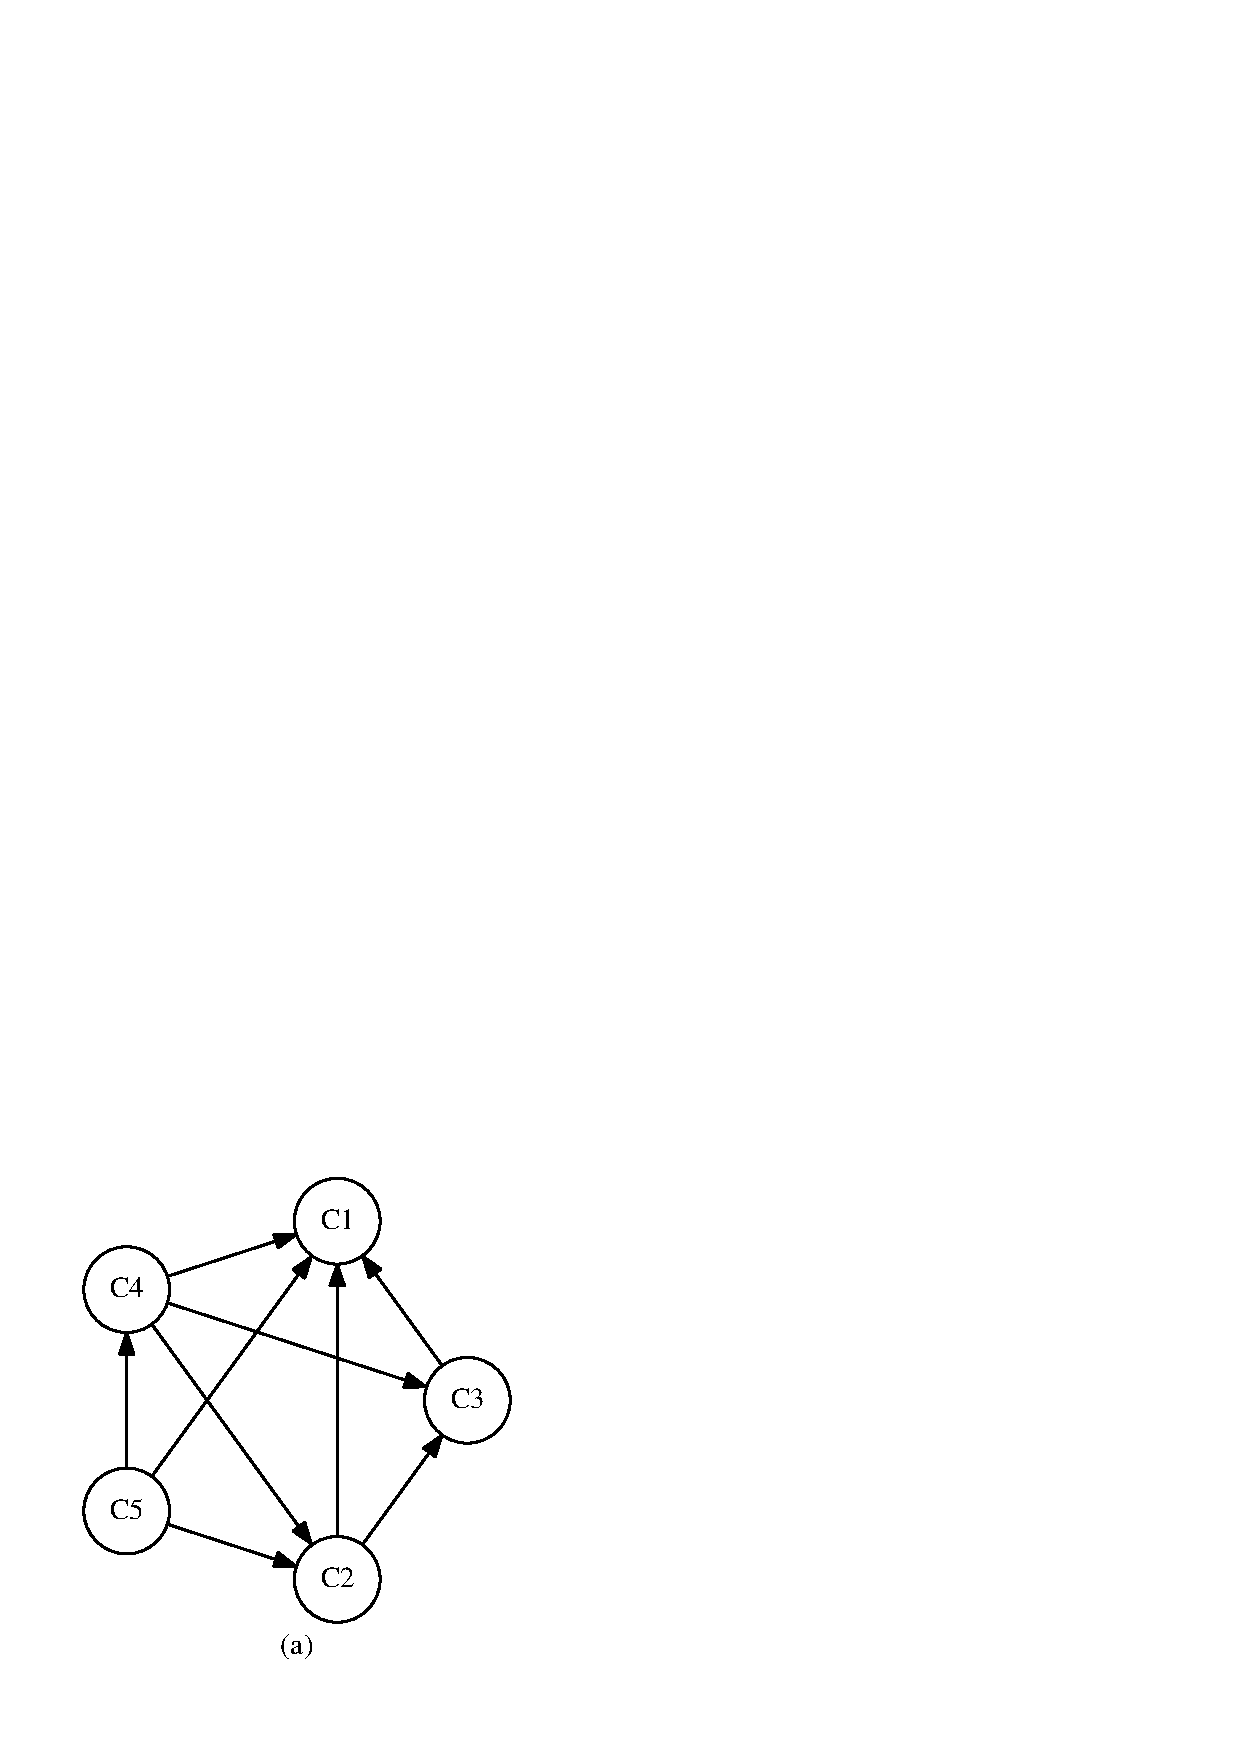
\includegraphics[width=0.42\columnwidth]{graphs/cart.pdf}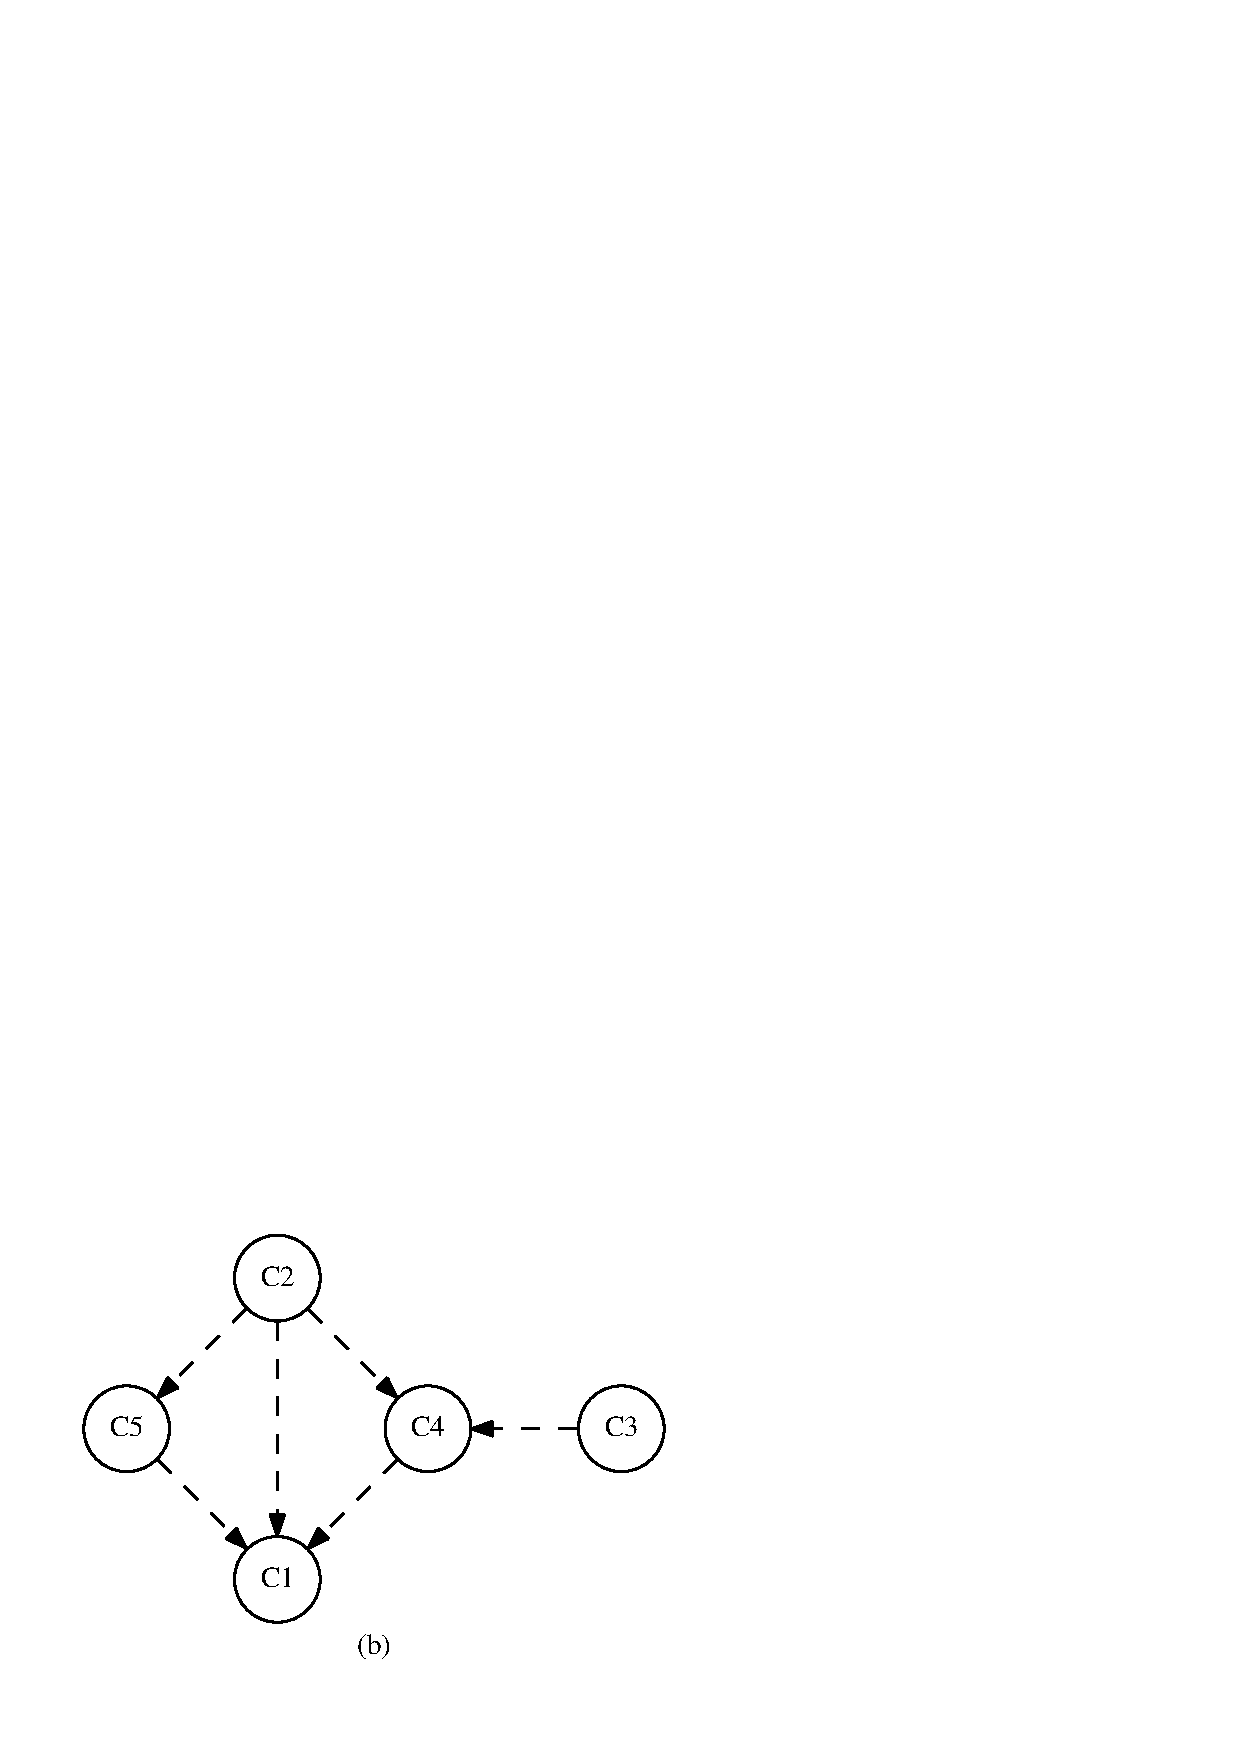
\includegraphics[width=0.57\columnwidth]{graphs/ccom.pdf}
\caption{Trend graphs for the CCC equivalence graph. Solid lines represent the artifact analysis. Dashed lines represent the understandability analysis.}
\label{fig:graphsforanalysis}
\end{figure}

\subsubsection{Building the Graphs}
In the community standards graph, we represent a directed edge from $C2 \rightarrow C1$ when  nPatterns(C1) $>$ nPatterns(C2) \emph{and}  nProjects(C1) $>$ nProjects(C2).
When there is a conflict between nPatterns and nProjects, as is the case between L2 and L3 where L2 is found in more patterns and L3 is found in more projects, an undirected edge is used.
This is to represent that there was no clear winner based on the two metrics used in the community standards analysis.
After considering all pairs of nodes in each equivalence class that also have an edge in Figure~\ref{fig:refactoringTree}, we have created a graph, for example Figure~\ref{fig:graphsforanalysis}a, that represents the frequency trends among the community artifacts. Note that with the CCC group, there is no edge between C3 and C5 because there is no straightforward refactoring between those representations, as discussed in Section~\ref{sec:refactoring}.

In the understandability graph, we represent a directed edge from $C2 \rightarrow C1$ when match(C1) $>$ match(C2) \emph{and} compose(C1) $>$ compose(C2). When there is a conflict between match and compose, as is the case with T1 and T3 where match(T1) is higher but compose(T3) is higher, an undirected edge is used. When one metric has a tie, as is the case with compose(C1) = compose(C5), we resort to the matching to provide the direction, in this case, C5 $\rightarrow$ C1. An example understandability graph is provided in Figure~\ref{fig:graphsforanalysis}b with the dashed arrows.
%\footnote{When there are confounded representations, as is the case with E8, E4, and E5 which all use tranformations from the CCC and the LIT equivalence classes, we omit those from the understandability graph. This makes sense since all use a transformation between T1 and T4 strongly favoring T1. }

\subsubsection{Topological Sorting}
Once the graphs are built for each equivalence class and each set of metrics, community standards and understandability, we apply a modified version of Kahn's topological sorting algorithm to obtain a total ordering on the nodes, as shown in Algorithm~\ref{topological}. In Kahn's algorithm, all nodes without incoming edges are added to a set $S$ (Line~\ref{addnoincomingtos}), which represents the order in which nodes are explored in the graph. For each $n$ node in $S$ (Line~\ref{beginwhile}), all edges from $n$ are removed and $n$ is added to the topologically sorted list $L$ (Line~\ref{addntoL}). If there exists a node $m$ that has no incoming edges, it is added to $S$.  In the end, $L$ is a topologically sorted list.

\begin{algorithm}
  \caption{Modified Topological Sort}\label{topological}
  \begin{algorithmic}[1]
\State  $L \gets$ []
\State $S \gets$ []
\State Remove all undirected edges (creates a DAG)
\State Add all disconnected nodes to $L$ and remove from graph. If there are more than one, mark the tie. \label{markTie1}
\State Add all nodes with no incoming edges to $S$. If there are more than one, mark the tie. \label{addnoincomingtos}
\While {$S$ is non-empty} \label{beginwhile}
	\State remove a node $n$ from $S$ \label{setn}
	\State add $n$ to $L$  \label{addntoL}
	\For {node $m$ such that $e$ is an edge from $n \rightarrow m$}
		\State remove $e$
		\If{$m$ has no incoming edges}
			\State add $m$ to $S$ \label{addToS}
		\EndIf
	\EndFor
	\State remove $n$ from graph
	\State If multiple nodes were added to $S$ in this iteration, mark those as a tie \label{markTie2}
\EndWhile
\State For all ties in $L$, use a tiebreaker.
  \end{algorithmic}
\end{algorithm}

One downside to Kahn's algorithm is that the total ordering is not unique. Thus, we mark ties in order to identify when a tiebreaker is needed to enforce a total ordering on the nodes. For example, on the understandability graph in Figure~\ref{fig:graphsforanalysis}b, there is a tie between C3 and C2 since both have no incoming edges, so they are marked as a tie on Line~\ref{markTie1}. Further, when $n=C2$ on line~\ref{setn}, both C5 and C4 are added to $S$ on Line~\ref{addToS}, thus the tie between them is parked on line~\ref{markTie2}. In these cases, a tiebreaker is needed.

Breaking ties on the community standards graph comes down to choosing the representation that appears in a larger number of projects, since it is more widespread across the community. Breaking ties in the understandability graph is trickier. Using Table~\ref{table:testedEdgesTable}, we compute the average matching score for all instances of each representation, and do the same for the composition score. For example, C4 appears in \todoLast{C2 -- C4}, \todoLast{C1 -- C4} and \todoLast{C3 -- C4} with an overall average matching score of 0.81 and composition score of 24.3. C5 appears in \todoLast{C1 -- C5} and \todoLast{C2 -- C5} with an average matching of 0.87 and composition of 28.28. Thus, C5 is favored to C4 and appears higher in the sorting.

After running the topological sort in Algorithm~\ref{topological}, we have a total ordering on nodes for each graph. After breaking ties as described, the topological sorts for all graphs are shown in Table~\ref{topologicalResults}.  For example, given the graphs in Figure~\ref{fig:graphsforanalysis}a and Figure~\ref{fig:graphsforanalysis}b, the topological sorts are {\tt C1 C3 C2 C4 C5} and {\tt C1 C5 C4 C2 C3}, respectively.

\begin{table*}
\centering
\caption{Topological Sorting, with the left-most position being highest \label{topologicalResults}}
\begin{tabular}{|| l || l || l || l || l || l ||}
				& CCC			& DBB 		& LBW & SNG & LIT \\ \hline
Community Standards		& C1 C3 C2 C4 C5 	& D2 D1 D3	&  L3 L2 L1 	& S2 S1 S3 	& T1 T3 T2 T4 \\
Understandability 			& C1 C5 C4 C2 C3 	& D3 D1 D2 	& L3 L2		& S2 S1		& T1 T2 T4 T3 \\
\end{tabular}
\end{table*}

\subsubsection{Summary}
There is a clear winner in each equivalence class, with the exception of DBB.
That is, the node sorted highest in the topological sorts for both the community standards and understandability analyses are C1 for CCC, L3 for LBW, S2 for SNG, and T1 for LIT.
After the top rank, it is not clear who the second place winner is in any of the classes, however, having a consistent and clear winner is evidence of a preference with respect to community standards and understandability.

This positive result, that the most popular representation in the corpus is also the most understandable, makes sense as people may be more likely to understand things that are familiar or well documented. However, while L3 is the winner for the LBW group, we note that L2 appears in slightly more patterns.

CCC and DBB are shuffled quite differently, and LBW and SNG don't have enough information from the understandability analysis since there is just one edge. DBB is an odd one as the orderings are completely reversed depending on the analysis.

%\begin{figure}[tb]
%\centering
%\includegraphics[width=\columnwidth]{illustrations/exampleUsage.eps}
%\vspace{-12pt}
%\caption{Example of one regex utilization}
%\vspace{-6pt}
%\label{fig:exampleUsage}
%\end{figure}









%\paragraph{CCC Group}
%This group is full of disagreement among the metrics. Five pairs were evaluated by all methods and only one pair, $C1 \Leftarrow C4$, has a somewhat clear winner with C1 (note that the matching metric is equivalent). All the others have disagreement between the community and understandability, or between the understandability metrics, matching and composition.
%
%
%\paragraph{DBB Group}
%D2 has the most community support appearing in nearly 14\% of the patterns, yet the understandability metrics favor both D1 and D3 over D2. The results are consistent across the board that D3 is always favorable to D1.
%
%\paragraph{LWB Group}
%
%\paragraph{LIT Group}
%
%\paragraph{SNG Group}
%
%=======
%\paragraph{CCC Group}
%This group is full of disagreement among the metrics. Five pairs were evaluated by all methods and only one pair, $C1 \Leftarrow C4$, has a somewhat clear winner with C1 (note that the matching metric is equivalent). All the others have disagreement between the community and understandability, or between the understandability metrics, matching and composition.
%
%
%\paragraph{DBB Group}
%D2 has the most community support appearing in nearly 14\% of the patterns, yet the understandability metrics favor both D1 and D3 over D2. The results are consistent across the board that D3 is always favorable to D1.
%
%\paragraph{LWB Group}
%\todoNow{Carl filling in these and adding some observations and context}
%
%\paragraph{LIT Group}
%
%\paragraph{SNG Group}
%
%>>>>>>> 61b90cac1ea534594cd76837430bc23ee51cc916




%
%(for rough draft...)
%
%Looks like M6 and M8 are the best meta-refactorings according to ANOVA.
%If you peek at MTResults Processing.csv on google docs, M6 has the best refactoring...every OCTAL type should be converted to an OR or preferably a CCC.
%
%M8 has a weak P value, but still ok in one case (0.12) and consistently says that 'aa*' should be written as 'a+'.
%
%Looks like M0, M1, M2, M3 and M9 are very dependent on the regex chosen, so regex-specific refactorings like:
%0.1401 \verb!&d([aeiou][aeiou])z'    &d([aeiou]{2})z'!
%0.075   \verb![\t\r\f\n ]'    [\s]'!
%0.1024  \verb![a-f]([0-9]+)[a-f]' [a-f](\d+)[a-f]'!
%0.1271  \verb![\{][\$](\d+[.]\d)[}]'!
%\verb!\\\{\\\$(\d+\.\d)\}'!
%(from M0,M1,M2,M9 respectively)
%
%have okay P-values and may indicate regex-specific refactorings, but do not indicate an overall trend for that type of refactoring.
%Notice that M3 does not even have a strong p-value candidate, but this may be thrown off because of the very confusing regex chosen for CCC:
%0.78    0.79
%\verb!xyz[_\[\]`\^\\]'!    \verb!xyz[\x5b-\x5f]'!
%which has a lot of escape characters, so that the hex group was easier to understand than the CCC.
%
%
%
%Meanwhile M4,M5 and M7 have both ambiguous p-values and anova results.  But this is still a finding: that no refactoring is needed between things like:
%\verb!(q4fab|ab)'! (\verb!(q4f){0,1}ab)'!
%\verb!tri[abcdef]3'!   \verb!tri(a|b|c|d|e|f)3'!
%\verb!&(\w+);'!    \verb!&([A-Za-z0-9_]+);'!
%(from M4,M5,M7 respectively)
%
%Although one refactoring from M5 might be of slight interest:
%0.1196  FALSE   \verb!tri[a-f]3'!  \verb!tri(a|b|c|d|e|f)3'!

%\todoMid{more data from the composition problems}


\section{Discussion}
\label{sec:discussion}

\subsection{Implications}

\paragraph{Coding Standards for Regexes}
Many organizations enforce coding standards in their repositories to ease understandability. 
Presently, we are not aware of coding standards for regular expressions, but this work suggests that enforcing standard representations for various regex constructs could ease comprehension. 

%A particular community (like Mozilla or some startup) may want to include regex refactoring into their coding standards.  We anticipate that having one preferred way to express a particular regex may increase regex understandability in the codebase for maintainers, leading to a reduction in errors related to misunderstanding regexes.

\paragraph{Other Refactorings}
The refactorings we suggest in this work are just a starting point as this is the first work to look 
at regex refactoring. 
Other refactorings exist that deserve further study, such as: 
\begin{description}
\item[Single line option]  \verb!'''(.|\n)+'''! is equivalent to \verb!(?s)'''(.)+'''!
\item[Multi line option]  \verb!(?m)G\n! is equivalent to \verb!(?m)G$!
\item[Multi line option]  \verb!(?i)[a-z]! is equivalent to \verb![A-Za-z]!
\item[Backreferences]  \verb!(X)q\1! is equivalent to \verb!(?P<name>X)q\g<name>!
\item[Word Boundaries]  \verb!\bZ! is equivalent to \verb!((?<=\w)(?=\W)|(?<=\W)(?=\w))Z!
\end{description}

\noindent This is not meant to be an exhaustive list as regex languages with richer feature sets may have even more equivalence classes available, but it provides a starting point. 

\paragraph{Migration Libraries} 
Other opportunities exist to improve the understandability of regexes in existing code bases
by looking for some of the less understandable regex representations, which can be thought of as antipatterns, and refactoring to the more common or understandable representations. Building migration libraries is another direction of future work to ease the manual burden of this process. 
%One terribly obvious application of our refactorings is to search existing codebases for regex patterns that are candidates for refactoring, allowing a person to quickly go through a list of possible changes and improve the understandability of the regexes in their codebase.

\paragraph{Finish me...}
Maintainers of code that is intentionally obfuscated for security purposes may want to develop regexes that they understand and then automatically transform them to equivalent but less understandable regexes.

One fundamental concept is when to use regexes for simple parsing, and when to write a full-fledged parser (for example, when parsing HTML).  Regexes that are trying to parse HTML, XML or similar languages could be refactored not into a better regex, but into some code with an equivalent intention that does parsing much better.

In our treatment, we have looked at all ranges as equivalent, all defaults as equivalent, and relied on many such generalizations.  By creating a much more granular model of regular expression refactorings (perhaps treating \verb!\d! and \verb!\w! quite separately), and making sure to carefully evaluate alternative representations of the most frequently used specific patterns (like \verb!\\s*! and \verb!.+!), many more strong and useful refactorings could be identified.



\subsection{Threats to Validity}

\subsubsection{Internal}
We measure understandability of regexes using two metrics, matching and composition. However, these measures may not reflect actual understanding of the regex behavior. For this reason, we chose to use two metrics and present the analysis in the context of reading and writing regexes, but the threat remains.

\todoMid{what about the threat of too few examples per node?}

We treated unsure responses as omissions and did not count those against the participants. Thus, if a participant answered two strings correctly with match/not match, and marked the other three strings as unsure, then this was 2/2 correct, not 2/5.

\subsubsection{External}
Participants in our survey came from MTurk, which may not be representative of people who read and write regexes on a regular basis.

The regexes we used in the evaluation were inspired by those commonly found in Python code, which is just one language that has library support for regexes. Thus, we may have missed opportunities for other refactorings based on how programmers use regexes in other programming languages.

Our community analysis only focuses on the Python language. Note that because the vast majority of regex features are shared across most general programming languages (e.g., Java, C, C\#, or Ruby), a Python {pattern} will (almost always) behave the same when used in other languages, whereas a utilization is not universal in the same way (i.e., it may not compile in other languages, even with small modifications to function and flag names).
As an example, the {\tt re.MULTILINE} flag, or similar, is present in Python, Java, and C\#, but  the Python {\tt re.DOTALL} flag is not present in C\# though it has an equivalent flag in Java.



\section{Conclusion}
In an effort to find smells that impact regex understandability, we created five equivalence class models and used these models to investigate the most common representations and most comprehensible representations per class.  
%We found the most common representations per class by both number of patterns and number of projects to be C1, D2, T1 and S2 (L3 has the most patterns, L2 has the most projects).
%We  identified three strongly preferred transformations between representations (i.e., $\overrightarrow{T4 T1}$, $\overrightarrow{D2 D3}$, and  $\overrightarrow{L2 L3}$). 
 The high agreement between the community standards and understandability analyses  suggests that one particular representation can be preferred over others in most cases.  
Based on these results, we recommend using hex to represent invisible characters in regexes instead of octal, and to escape special characters with slashes instead of wrapping them in brackets.  
Further research is needed into more granular models that treat common specific cases separately.
%, and that address the effect of length on understandability when transforming from one representation to another.




\begin{table*}\begin{small}\begin{center}\caption{Averaged Info About Edges}\label{table:testedEdgesTable}\begin{tabular}
{llccccccc}
Index & Representations & Pairs & Match1 & Match2 & $H_0: \mu_{match1} = \mu_{match2}$ & Compose1 & Compose2 &  $H_0: \mu_{comp1} = \mu_{comp2}$ \\
\toprule[0.16em]

E8 & C2,T4 -- C5,T1 & 2 & 0.60 & 0.82 & <0.001 & 11.0 & 29.0 & <0.001\\

E16 & T1 -- T4 & 2 & 0.80 & 0.60 & 0.001 & 26.0 & 11.0 & <0.001\\

E5 & C1,T4 -- C2,T1 & 2 & 0.81 & 0.86 & 0.383 & 15.5 & 27.5 & <0.001\\
E4 & C1,T2 -- C2,T1 & 2 & 0.84 & 0.86 & 0.934 & 19.5 & 27.5 & <0.001\\


E12 & D2 -- D3 & 2 & 0.78 & 0.87 & 0.011 & 26.5 & 29.0 & 0.085\\
E13 & L2 -- L3 & 3 & 0.86 & 0.91 & 0.032 & 27.3 & 29.3 & 0.052\\
\hline
E6 & C2 -- C4 & 1 & 0.83 & 0.92 & 0.075 & 18.0 & 20.0 & 0.601\\
E10 & D1 -- D2 & 2 & 0.84 & 0.78 & 0.120 & 28.0 & 26.5 & 0.347\\
E1 & C1 -- C2 & 2 & 0.94 & 0.90 & 0.121 & 28.0 & 27.0 & 0.514\\
E3 & C1 -- C5 & 2 & 0.94 & 0.90 & 0.287 & 28.0 & 28.0 & 1.000\\
E15 & T1 -- T3 & 3 & 0.88 & 0.86 & 0.320 & 21.7 & 22.7 & 0.613\\
E11 & D1 -- D3 & 2 & 0.84 & 0.87 & 0.349 & 28.0 & 29.0 & 0.408\\
E2 & C1 -- C4 & 6 & 0.87 & 0.84 & 0.352 & 25.8 & 25.0 & 0.465\\
E17 & T2 -- T4 & 2 & 0.84 & 0.81 & 0.498 & 19.5 & 15.5 & 0.141\\
E9 & C3 -- C4 & 2 & 0.61 & 0.67 & 0.593 & 22.5 & 24.5 & 0.379\\
E7 & C2 -- C5 & 4 & 0.85 & 0.86 & 0.602 & 26.5 & 28.5 & 0.063\\
E14 & S1 -- S2 & 3 & 0.85 & 0.86 & 0.776 & 26.3 & 27.0 & 0.638\\



\bottomrule[0.13em]\end{tabular}\end{center}\end{small}\end{table*}


\begin{table*}\begin{small}\begin{center}\caption{some Group table caption}\label{table:groupANOVATable}\begin{tabular}
{lcc}
group & Pregex & Prefactoring \\
\toprule[0.16em]
CCC-LIT & 0.000000001 & 0.000030400\\
CCC & 0.000000000 & 0.427400000\\
DBB & 0.591100000 & 0.072200000\\
LIT & 0.000000000 & 0.000105000\\
LWB & 0.989700000 & 0.041200000\\
SNG & 0.000037600 & 0.958000000\\
\bottomrule[0.13em]\end{tabular}\end{center}\end{small}\end{table*}


\balance

\section*{Acknowledgements}
This work is supported in part by  NSF SHF-EAGER-1446932.


\bibliographystyle{IEEEtran}
\bibliography{biblio,stolee}

\end{document}

